\section{System Calls}


\begin{frame}{API del Sistema Operativo}
  \begin{itemize}
  \item Los SOs proveen un conjunto de interfaces mediante las cuales un proceso que corre en espacio de usuario accede a un conjunto de funciones comunes
   \begin{center}
    \fbox{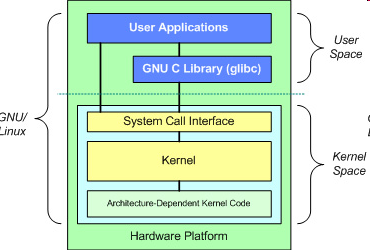
\includegraphics[width=0.4\textwidth]{images/layers.png}}
   \end{center}

  \item En UNIX el API principal que provee estos servicios es libc:
  \begin{itemize}
    \item Es el \alert{API} principal del SO
    \item Provee las librerías estandar de C
    \item \textit{Es una Interface entre aplicaciones de usuario y las \alert{System Calls}(System Call Wrappers).} 
      \end{itemize} 
  \end{itemize}
\end{frame}

\begin{frame}{POSIX APIs}
  \begin{itemize}
  \item La funcionalidad anterior está definida por el estandar POSIX
  \item Su próposito es proveer una interfaz común para lograr portabilidad
  \item En el caso de las System Calls, el desarrollador generalmente interactúa con el \textit{API} y NO directamente con el Kernel   
  \item En UNIX por lo general cada función del \alert{API} se corresponde con una \alert{System Call}
  \end{itemize}
 \begin{center}
    \fbox{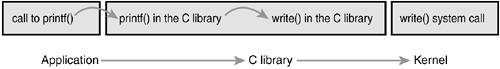
\includegraphics[width=0.8\textwidth]{images/printf.jpg}}
   \end{center}
\end{frame}

\begin{frame}{System Calls - Repaso}
  \begin{itemize}
  \item Son llamados al kernel para ejecutar una función específica que controla un dispositivo o ejecuta una instrucción privilegiada 
  \item Su próposito es proveer una interfaz común para lograr portabilidad
  \item Su funcionalidad la ejecuta el Kernel   
  \item Recordar  
  \begin{itemize}
    \item Cambio de Modo
    \item ¿Como se pasa de modo usuario a modo Kernel?
  \end{itemize} 

  \end{itemize}
 
\end{frame}

\begin{frame}{Invocando System Calls}
  \begin{itemize}
  \item Utilizando los wrappers de glibc
         \begin{itemize}
            \item \texttt{int rc = chmod( ``/etc/passwd'' , 0444);}
         \end{itemize}
  \item Invocación explícita utilizando la System Call \alert{syscall} provista por glibc
         \begin{itemize}
            \item Definida en la libreria unistd.h
            \begin{itemize}
            \item \texttt{long int syscall (long int sysno, …) }
	    \end{itemize} 
	    \item Ejemplo utilizando syscall: 
              \begin{itemize}
                \item \texttt{rc = syscall(SYS\_chmod, ``/etc/passwd'', 0444);}
              \end{itemize}
         \end{itemize} 
  \end{itemize}
\end{frame}

\begin{frame}[fragile]
\frametitle{Ejemplo}
\lstset{language=C,
                basicstyle=\ttfamily,
                keywordstyle=\color{blue}\ttfamily,
                stringstyle=\color{red}\ttfamily,
                commentstyle=\color{green}\ttfamily,
                morecomment=[l][\color{magenta}]{\#}
}
\begin{lstlisting}
#include <stdlib.h>
#include <sys/syscall.h>
#include <sys/time.h>
#include <unistd.h>
#define SYS_gettimeofday 78

void main(void){
   struct timeval tv;
   /* usando el wrapper de glibc */
   gettimeofday(&tv, NULL);

   /* Invocación explícita del  system call */
   syscall(SYS_gettimeofday, &tv, NULL);
}
\end{lstlisting}
\end{frame}


\begin{frame}{Interrupciones y System Calls}
  \begin{itemize}
    \item La manera en que una system call es llevada a cabo dependerá del procesador.
      \begin{itemize}
	    \item \texttt{Los procesadores x86 se basan en el mecanismo de interrupciones}.
	\end{itemize}  
    
   \item Interrupción enmascarable int 0x80 en Linux.
   \begin{itemize}  
   \item \texttt{Se usa el vector 0x80 para transferir el control al kernel. Este vector de interrupción esta inicializado durante el startup del sistema.}
 \end{itemize}
    \item Una librería de espacio de usuario(libc) carga el índice de la system call y sus argumentos, la interrupción enmascarable por software 	0x80 es invocada, la cual resulta en el cambio de modo.	
   \item A través de la estructura sys\_call\_table y el registro eax como índice se determina que \emph{handler function} invocar.
  \end{itemize}
\end{frame}

\begin{frame}[fragile]
\frametitle{System Calls e Interrupciones}
\lstset{language=C,
                basicstyle=\ttfamily,
                keywordstyle=\color{blue}\ttfamily,
                stringstyle=\color{red}\ttfamily,
                commentstyle=\color{green}\ttfamily,
                morecomment=[l][\color{magenta}]{\#}
}
Consideremos el siguiente caso:
\begin{lstlisting}
#include <syscall.h>
#include <unistd.h>
#include <stdio.h>
#include <sys/types.h>
#define sys_getpid 20
int main(void) {
  long ID = syscall(SYS_getpid);
  printf ("El pId del proceso es:\n", ID);
}
\end{lstlisting}
\end{frame}

\begin{frame}[fragile]
\frametitle{System Calls e Interrupciones(cont.)}
\lstset{language=C,
                basicstyle=\ttfamily,
                keywordstyle=\color{blue}\ttfamily,
                stringstyle=\color{red}\ttfamily,
                commentstyle=\color{green}\ttfamily,
                morecomment=[l][\color{magenta}]{\#}
}
El compilador generará:
\begin{lstlisting}
_setuid:
subl $4,%exp
pushl %ebx
movzwl 12(%esp),%eax
movl %eax,4(%esp)
movl $20,%eax
movl 4(%esp),%ebx
int $0x80
movl %eax,%edx
testl %edx,%edx
jge L2
negl %edx
movl %edx,_errno
movl $-1,%eax
popl %ebx
addl $4,%esp
ret
L2:
movl %edx,%eax
popl %ebx
addl $4,%esp
ret

\end{lstlisting}
\end{frame}

\begin{frame}{System Calls en GNU Linux}
   \begin{itemize}  
   \item Debemos declarar nuestra syscall por un número único(syscall number). 
   \item Agregamos una entrada a la syscall table.
   \item Debemos considerar el sys call number.
   \item Ver que el código fuente organizado por arquitectura.
   \item Respetar las convenciones del Kernel(ej. prefijo sys\_).
 \end{itemize}

\begin{block}{/usr/src/linux-3.8/arch/x86/entry/syscalls/syscall\_32.tbl}
  \begin{block}{}
     343     i386    clock\_adjtime            sys\_clock\_adjtime    \\           
     347     i386    process\_vm\_readv        sys\_process\_vm\_readv  \\          
     348     i386    process\_vm\_writev       sys\_process\_vm\_writev \\          
     349     i386    kcmp                      sys\_kcmp \\
     350     i386    finit\_module             sys\_finit\_module \\
     \alert{351     i386    newcall                   sys\_newcall} \\ 
  \end{block}

\end{block}

\end{frame}


\begin{frame}{System Calls en GNU Linux(Cont.)}
   \begin{itemize}  
   \item Debemos definir el prototipo de nuestra system call 
   \item Los parámetros a system calls deben ser realizados por medio del stack
   \item Informamos de esto al compilador mediante la macro asmlinkage
    \begin{itemize}
	 \item \alert{asmlinkage} instruye al compilador a pasar parámetros por stack y no 
          por ejemplo en registros 
    \end{itemize}   
 \end{itemize}

\begin{block}{/usr/src/linux-3.8/include/linux/syscalls.h}
asmlinkage long sys\_newcall(int i);

\end{block}

\end{frame}

\begin{frame}{System Calls en GNU Linux(Cont..)}
   \begin{itemize}  
   \item Debemos nuestra syscall en algún punto del árbol de fuentes. 
   \item Podemos utilizar algún archivo existente.
   \item Podemos incluir un nuevo archivo y su correspondiente Makefile. 
   \begin{itemize}
	 \item \alert{Ver apuntes adjuntos} 
    \end{itemize}   
 \end{itemize}

\begin{block}{En algún archivo ya incluido en los fuentes del Kernel...}
asmlinkage int sys\_newcall(int a) { \\
	printk(``calling newcall... '');   \\
return a+1; \\
}
\end{block}
   \begin{itemize}
	 \item \alert{¿printk?}, ¿porque no printf? 
    \end{itemize}   

\end{frame}

\begin{frame}{System Calls en GNU Linux(Cont...)}
   \begin{itemize}  
   \item \textbf{Recompilar el Kernel!}
    \begin{itemize}
	 \item Idem Práctica 2 
    \end{itemize}   
 \end{itemize}
\end{frame}


\begin{frame}[fragile]
\frametitle{Invocando explícitamente nuestra System Call}
\lstset{language=C,
                basicstyle=\ttfamily,
                keywordstyle=\color{blue}\ttfamily,
                stringstyle=\color{red}\ttfamily,
                commentstyle=\color{green}\ttfamily,
                morecomment=[l][\color{magenta}]{\#}
}

\begin{lstlisting}
#include <linux/unistd.h>
#include <stdio.h>
#define sys_newcall 351
int main(void) {
  int i = syscall(sys_newcall,1);
  printf ("El resultado es:\n", i);
}
\end{lstlisting}
\end{frame}


\begin{frame}{Strace}
   \begin{itemize}  
    \item \textbf{Reporta las system calls que realiza cualquier programa}
    \item man strace
    \item Opción útil -f (tiene en cuenta procesos hijos)  
 \end{itemize}
\begin{block}{strace a.out (hola mundo)}
execve("./a.out", ["./a.out"], [/* 62 vars */]) = 0 \\
brk(0)                                  = 0x1295000 \\
access("/etc/ld.so.nohwcap", F\_OK)      = -1 ENOENT (No such file or directory)\\
mmap(NULL, 8192, PROT\_READ|PROT\_WRITE, MAP\_PRIVATE|MAP\_ANONYMOUS, -1, 0) = 0x7f3b70b43000\\
access("/etc/ld.so.preload", R\_OK)      = -1 ENOENT (No such file or directory)\\

\end{block}
\end{frame}

\begin{frame}
\frametitle{DESAFIO}
   \begin{itemize}  
   \item Realizar un parche que contenga los cambios asociados a la siguiente \textit{system call}: 
   \begin{itemize}
      \item Simplemente debe imprimir el texto ``Hello World!'' a través de la función \textit{printk}
      \item Se debe hacer sobre la la \emph{4.4.6}
    \end{itemize}
    \item Tips:
    \begin{itemize}
      \item Utilizar explicación y práctica para guiarse      
      \item \url{http://lxr.free-electrons.com/}
    \end{itemize}
 \end{itemize}
\end{frame}

\begin{frame}[fragile]
\frametitle{DESAFIO - Implementación}
  \begin{itemize}
    \item ¿Dónde incluir la implementación?:
    \begin{itemize}
      \item Dos opciones:
      \begin{itemize}
        \item Incluir el código en un fichero existente
        \item Agregar un nuevo fichero $\rangle$ modificar \emph{Makefile} existente
      \end{itemize}
    \end{itemize}
    \item Crearemos un nuevo fichero \emph{.c} nuevo en \emph{kernel/mysyscall.c}
  \end{itemize}
  \begin{lstlisting}
#include <linux/syscalls.h> /* For SYSCALL_DEFINEi() */
#include <linux/kernel.h>

SYSCALL_DEFINE0(mysyscall)
{
  printk(KERN_DEBUG "Hello world\n");
  return 0;
}      
  \end{lstlisting}
\end{frame}

\begin{frame}[fragile]
\frametitle{DESAFIO - Modificar \emph{Makefile}}
  \begin{lstlisting}
#
# Makefile for the linux kernel.
#

obj-y = ...
        async.o range.o groups.o smpboot.o mysyscall.o
...
  \end{lstlisting}  
\end{frame}

\begin{frame}[fragile]
\frametitle{DESAFIO - Test}
  \begin{lstlisting}
#include <linux/errno.h>
#include <sys/syscall.h>
#include <linux/unistd.h>
#include <stdio.h>

#define __NR_MYSYSCALL -num-syscall-

int main() {
  printf("Invocando system call\n");
  return syscall(__NR_MYSYSCALL);
}
  \end{lstlisting}  
\end{frame}


\begin{frame}[fragile]
\frametitle{DESAFIO - Parche}
  \begin{lstlisting}
## Crear parche
$ diff -urpN ${DIR_KERNEL_ORIGINAL} ${DIR_KERNEL_MODIFICADO} > patch-4.4.6-so2016

## Aplicar parche
$ patch -p1 < ${RUTA_MI_PARCHE}
  \end{lstlisting}  
\end{frame}

%%% Local Variables: 
%%% mode: latex
%%% TeX-master: "main"
%%% End:
